\documentclass[11pt]{article}
\usepackage{xspace}
\usepackage{palatino}
\usepackage{fancyhdr}
\usepackage{graphicx}
\usepackage[headings]{fullpage}
\pagestyle{fancy}
\newcommand\STex{Simple\TeX\xspace}
\newcommand\LTex{\LaTeX\xspace}
\lhead{\begin{slshape}Justin Bailey\end{slshape}}
\chead{\begin{slshape}\copyright\ 2010 \STex\end{slshape}}
\rhead{\begin{slshape}\today\end{slshape}}
\fancypagestyle{first}{\fancyfoot{}} % No page numbers
\renewcommand\floatpagefraction{0.8} 
\begin{document}
\thispagestyle{first}
\begin{center}
\Huge{\STex: Architectural Overview}
\end{center}

The \STex architecture has six components:

\begin{itemize}
\item \textbf{Web} -- Stateless servers, running (J)Ruby on Rails, for
  managing application UI. Also handles file upload/download.
\item \textbf{Database} -- Handles user information, document
  structure, and permissions.
\item \textbf{\LTex Processors} -- Stateless servers responsible for
  generating PDF documents from \LTex source. As demand increases more
  servers can be brought online.
\item \textbf{EtherPad Servers} -- Hosts EtherPad instances. As demand
  increases more can be provisioned.
\item \textbf{Load Listener} -- Monitors load of \LTex and EtherPad
  servers, and can provision additional servers if needed. Also able
  to remove servers as load decreases.
\item \textbf{Message Bus} -- Implemented via Simple Queue Service
  (SQS). All requests for \LTex processing, EtherPad instances, and
  other as-yet-undetermined resources from the web servers will be
  mediated by the message bus.
\end{itemize}

Figure \ref{fig_arch} shows the relationships between these
components.

\begin{figure}[h]
\centering
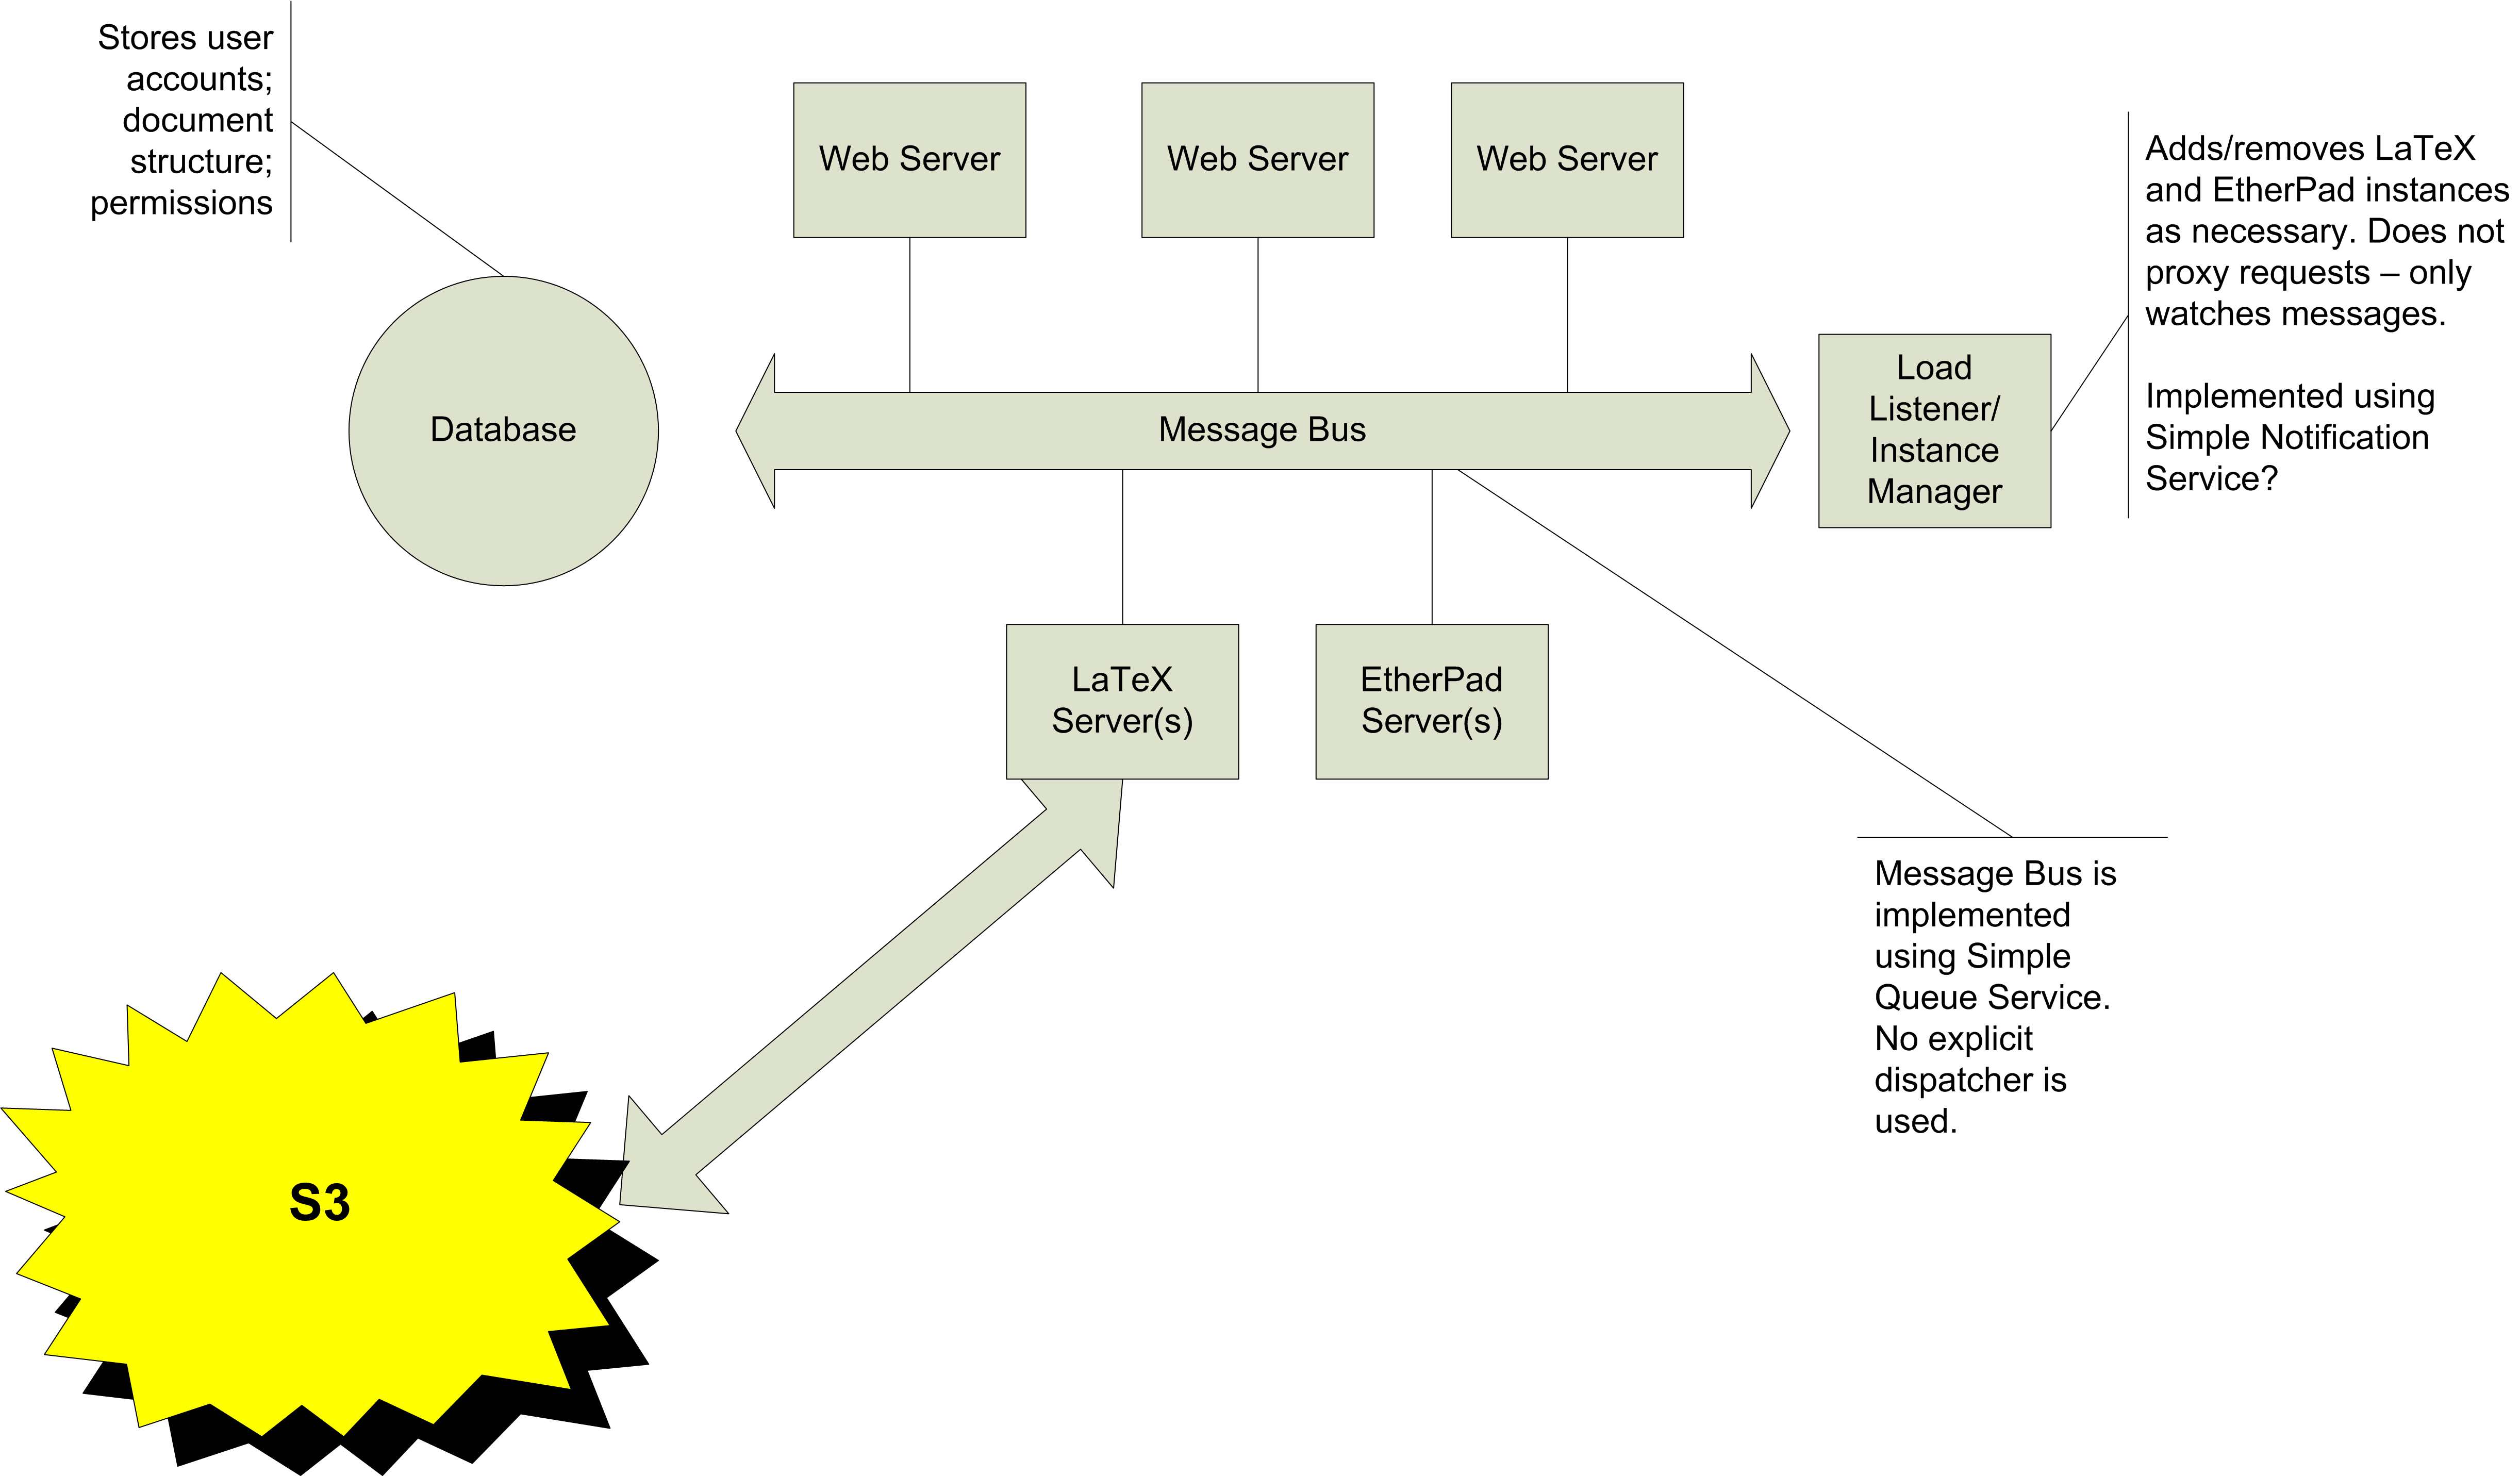
\includegraphics[width=6in,height=3.3738in]{SimpleTexArchitectureDiagram}
\caption{Initial sketch of the \STex architecture.}
\label{fig_arch}
\end{figure}

\STex is built around documents -- managing and creating PDF files
from \LTex source. Users own documents and invite others to
collaborate, but the \STex does not manage its work based on users. It
manages based on documents.

\section{\LTex Processors}

Each \LTEx processor (Figure \ref{fig_arch}) watches the message bus
for document processing requests. SQS ensures that only one server at
a time will read a given request. The server will follow these steps
once it receives a request:\footnote{Error handling and timeout issues
  are left out but also must be dealt with.}

\begin{enumerate}
\item \textbf{Visibility} -- Set the visibility timeout on the message
  to five minutes. This gives the server time to process the
  document.\footnote{We'll need to manage long-running documents. Five
    minutes probably indicates an error, but could be legitimate for
    long documents. Possibly a premium pricing thing?}.
\item \textbf{Document files} -- All files related to the given document are retrieved from storage and placed on the server. This includes custom packages and files.
\item \textbf{\LTex} -- \LTex is run on the document and the output is placed back into storage.
\item \textbf{Notification} -- The \LTex processor sends a notification that the document has finished processing and looks for another document to process.
\end{enumerate}

Each \LTex processor is identical to the others. They have Linux
installed, can run \LTex, have a default set of packages installed,
and can interact with Amazon's services (e.g., SQS, S3, etc.). They do
not have user accounts for each \STex user. 

\subsection{Document Security During Processing}

Keeping users documents separate and isolated during processing
requires special handling. In a normal UNIX environment, file system
permissions keep users from reading each other's documents. 

\STex
cannot rely on file system permissions because the number of \STex
users could grow very large. Additionally, keeping all \LTex
processors synchronized with the latest set of user accounts would be
difficult. \STex will instead use the following scheme:

\begin{itemize}
\item Each server will have 20 users (\texttt{nobody1} --
  \texttt{nobody20}) which cannot login interactively.
\item A scratch directory will exist on each server. No one except
  root will be able to read or modify the directory.
\item After receiving a request to create a document, the server will
  select a \texttt{nobody} to run the job. The \texttt{nobody} selected will not currently
  be running any jobs, and no jobs will be started while the \texttt{nobody} is
  ``busy.''
\item A randomly-named directory which only the selected
  \texttt{nobody} can access will be created under the scratch
  directory. An existing directory will \emph{never} be re-used.
\item The files necessary for the job will be copied from storage and
  placed in the new directory. 
\item \LTex will be started in a new process, running as that user,
  configured to use the new directory.
\item When finished, the final document will be retrieved
  and placed in storage. The directory will then be
  deleted.
\end{itemize}

This scheme ensures that no document can read files attributed to
another document. The scratch directory can only be accessed by root,
which ensures the \texttt{nobody} users cannot list its contents. Even
knowing the name of another directory will not help, since different
\texttt{nobody} user's own them. Finally, if the names chosen are
truly random, it will be impossible to guess the name of another
directory owned by the same \texttt{nobody}.

\subsubsection{Limitations}

This solution requires that the files for each document are copied from
storage each time the document is processed. This will work fine if a document
is only processed once a day, or even a few times an hour. It will not work very well when a document is processed repeatedly. Bandwidth usage and
transfer time could be prohibitive. 

\end{document}
